 \documentclass[aps,pre,showpacs,twocolumn]{revtex4}
\usepackage{amssymb}
\usepackage{graphicx}
\usepackage{epstopdf}
\usepackage{colordvi}
\usepackage{color}
\usepackage{dcolumn,amsmath,amsthm,amscd,amsfonts,amssymb,epsfig,graphics,graphicx,eucal}
\usepackage[dvipsnames]{xcolor}
\usepackage{comment}
\usepackage[section]{placeins}
\pdfoutput=1
\newcommand{\PT}{{\cal PT}}
\newcommand{\sn}{\mbox{sn}}
\newcommand{\dn}{\mbox{dn}}
\newcommand{\tomega}{\tilde{\omega}}
\DeclareMathOperator{\sech}{sech}

\begin{document}

\title{Localized modes in saturable Kerr media embedded in non-$\PT$-symmetric complex localized potentials}

\author{F. C. Moreira$^{1}$, S. B. Cavalcanti$^{1}$ }

\affiliation{
$^1$Universidade Federal de Alagoas, Campus A. C. Sim\~oes - Av. Lourival Melo Mota, s/n, Cidade Universit\'aria, Macei\'o - AL 57072-900, Brazil}

\date{\today}

\begin{abstract}
One-dimensional nonlinear wave propagation in a medium whose  refractive index is represented by a local non-${\cal PT}$ complex  potential, is theoretically investigated. We report on the existence of families of stable asymmetric spatial solitons in a saturable nonlinear medium in the presence of a gain/loss asymmetrical profile.  A tunable parameter defines the deviation from the ${\cal PT}- $symmetric case, and a thorough study on the existence and stability of soliton families is carried out. The properties of the nonlinear modes bifurcating  from the eigenvalue of the underlying linear problem are investigated. We obtain the remarkable result that even within an asymmetrical profile one still may obtain families of stable solitons below and above the phase transition where a collision between two real eigenvalues of the linear equation bifurcates into a pair of complex eigenvalues. The eigenvalue ranges in the power-eigenvalue diagrams  for different gain/loss profiles are inspected and, it is found that the saturable nonlinearity severely restricts these ranges as the eigenvalues tend quite fast to an asymptotic profile as power increases. Examples of the dynamics of the asymmetric solitons obtained by numerical simulations are shown to agree quite well with the analytical results.
\end{abstract}
\pacs{42.65.Tg, 42.65.Sf }
\maketitle

%\input{epsf.tex}

%\epsfverbosetrue

\section{Introduction}

The past decade has witnessed an intense activity in linear optical systems, described by non-Hermitian Hamiltonians, triggered
by reports on a wide class of complex potentials that obeys the  parity-temporal symmetry, the well known $\PT$ symmetry~\cite{Bender1}. 
In spite of being non-Hermitian, these $\PT$-symmetric Hamiltonians exhibit real spectra, and also are probability conservative systems.  These 
Hamiltonians fit perfectly $\PT$-symmetric optical structures through the association of the local potential function with complex-valued refractive index profiles \cite{Ruter2010,peschel,peng}. This association 
has been quite fruitful and has turned the field of optics to be a particularly adequate ground to test the amazing consequences of $\PT$-symmetric systems \cite{Guo,Longhi,Makris}. One of these is the onset of a phase transition related to the spontaneous symmetry breaking that occurs when the rate between the real and imaginary parts of the refractive index reaches a critical point. As a result, the all-real spectrum undergoes a phase transition to the complex plane. This phase transition has been observed and applied to a number of devices based on $\PT$ optical systems \cite{feng2013,feng2014,science14}. 

The interplay between nonlinearity with gain/loss is even a more interesting problem with striking consequences. For example, it has been reported that $\PT$-symmetric nonlinear optical media supports the unexpected possibility of soliton propagation \cite{Christodoulides1}. Further novel properties have been actively explored in recent years \cite{malomed11,konotop12,yang12,segev13,ulf15}.  
 
The developments reported in $\PT$-symmetric optical structures have also triggered further studies 
to include non-$\PT$-symmetric complex potential functions widening 
the potentiality of $\PT$ symmetry 
features such as a real spectra as well a phase transition ~\cite{Cannata1998,Miri2013,Tsoy2014, Yang2016}. These potentials contain
free parameters that represent tuning. By tuning the refractive index below a critical value the real spectrum undergoes a phase transition 
to the complex plane. By adding a real 
part with an adjustable parameter 
one opens a tunable
possibility with ranges that admits real spectra and also a phase transition to the complex phase. 

Nonlinear Kerr systems have been studied in a non-$\PT$-symmetric 
potential and the continuous families of nonlinear modes reported 
there are attributed to a conserved quantity, in the sense that it 
does not vary with the transverse spatial coordinate $x$ \cite{npt_solitons} and thus, reflects a content of 
symmetry in the system. Recently, we have studied the existence and stability of solitons in quadratic nonlinear unidimensional media 
under the influence of a one-parameter family asymmetric class of potentials \cite{Yang2016} and found families of stable solitons \cite{moreira16} bifurcating from the fundamental mode as well as 
from the second harmonic. However, to the best of our knowledge, higher nonlinearities in non-$\PT$-symmetric systems have
not been investigated. Materials with high nonlinear coefficients 
such as semiconductor doped glasses and organic polymers, cannot be described by a Kerr-type nonlinearity \cite{gatz}, as in these 
materials, the saturation of the nonlinear refractive index occurs at moderately high pulse 
intensities so that one must include the effect of higher order nonlinearities. Furthermore, theoretical and experimental results have indicated that a saturable nonlinear medium is suitable for the propagation and control of spatial solitons. As a notorious example, photorefractive optical solitons which can be induced at relatively low power formation are quite important for applications in all-optical switching and signal processing \cite{Segev}. 

 Considering the generalization of the class of functions $V(x)$ 
 (presented in \cite{Yang2016}) that 
 admit stable nonlinear modes, in the present work we study saturable nonlinear optical waveguides described by a class of tunable complex potentials which are not $\PT$-symmetric. The basic motivation to study 
 this type of tunable
 potential lies on the fact that this additional asymmetry parameter
 widens the scope of non-Hermitian Hamiltonians with real spectra,
 besides the effects that a saturable nonlinearity may reveal, 
 paving the way for new metamaterials with designed properties. 
 We find that this class of tunable asymmetric potentials 
 admits stable localized modes whose properties are quite modified by 
 the saturable nonlinearity. The properties of nonlinear modes are investigated, revealing interesting results on the influence of the
 asymmetry on the existence and stability of localized solutions which 
 we now, proceed to describe: in Sec. II we present the model and 
 statement of the problem. Sec. III presents briefly the linear 
 properties of the the  complex potential. Section IV is devoted to the existence of stable solitons while in section V their stability and dynamic are investigated. Finally, in Sec. VI we  conclude and 
 discuss the results obtained. 
 
 
\section{Theoretical Model}
Let us begin by writing the propagation equation of an optical field $u(\xi,\zeta)$ through a diffractive nonlinear saturable medium:

\begin{equation}
    i\frac{\partial u}{\partial\zeta}+\frac{\partial^{2}u}%
{\partial\xi^{2}}+\left[ g^2+\alpha g+i g_\xi \right]
u
+\sigma \frac{|u|^2}{1+\gamma|u|^2}u=0
\label{final}
\end{equation}
$u$ being the dimensionless amplitude of the field  while $\xi$ and $\zeta$ are, respectively, dimensionless transverse and propagation coordinates, scaled to the characteristic size of a localized 
modulation of the refractive index which is fully described by a real function $g\equiv g(\xi)$. 
The real part being $g^2+\alpha g$, where $\alpha$ is a free parameter which plays the role of a relative strength of the 
real part of the potential to the imaginary part, which is defined as:  $g_{\xi}\equiv\frac{dg}{d\xi}$. This adjustable parameter $\alpha$, widens the scope of non-Hermitian Hamiltonians with real spectra and may allow the breaking of the real spectrum \cite{Yang2016}. Fig.  \ref{fig:FF_phasebreak} (top right panel) shows the variation of the real part $g^2 + \alpha g$ as a function of $\alpha$ illustrating its effect on the amplitude of the real part of the potential function. The last term 
in equation ($\ref{final}$) represents a saturable third order nonlinear  material with saturation parameter $\gamma$, with $\gamma=0$ representing the usual Kerr nonlinearity without saturation. The nonlinearity may be of a self-focusing $(\sigma > 0)$ or a self-defocusing type, ($\sigma < 0$).

We look 
for localized solutions of ($\ref{final}$) in the form,
\begin{equation}
u\left(  \xi,\zeta\right)  =w\left(  \xi\right)  e^{ib\zeta}, ,\label{statio}%
\end{equation}
where $b$ is the soliton propagation constant and  $w(\xi)$  is the solution of
\begin{equation}
\frac{d^{2}w}{d\xi^{2}}+\left[ g^2+\alpha g+i g_\xi -b\right]  w+\sigma \frac{|w|^2}{1+\gamma |w|^2}w,
\label{stat}
\end{equation}
subject to zero boundary conditions $ w\left(  \xi\right)\to 0 $ as $|\xi|\to \infty$.
\section{Linear properties of the asymmetric localized potential}
Previous work \cite{Yang2016} has shown that, similarly to the $\PT$-symmetric case, the complex potential
\begin{equation}
G(\xi,\alpha)=g^2+\alpha g +ig_\xi
\end{equation}
when substituted into the linear version of equation (\ref{stat}), that is, 
\begin{equation}
Lw=b_1w,
\label{npt_linear}
\end{equation}
where $b_1$ is the linear eigenvalue and the operator $L$ is defined as 
\begin{equation}
L=\frac{d^2}{d\xi^2}+G,
\label{lineareqs}
\end{equation}


\noindent depending on the value of $\alpha$, may exhibit all-real spectrum. Furthermore it was proved, for sufficiently mild conditions, that $\alpha=0$ always guarantees a real spectrum for (\ref{lineareqs}). Let us now briefly describe the
recently reported \cite{moreira16} linear properties of (\ref{lineareqs}) when the potential $G$ is generated from the following function:
\begin{equation}
g=V\sech{\left[1+\beta\left(\frac{1+\tanh(\xi)}{2}\right)\right]\xi},
\label{gform}
\end{equation}
where the constant $V$ is the amplitude and the constant $\beta$ is its degree of asymmetry. The function $g$ is continuously differentiable, has a global maximum at $\xi=0$ and is asymmetric for $\beta\neq 0$, as is illustrated in Fig. \ref{fig:FF_phasebreak}. The function $g$ decays as $e^{\xi}$ when $\xi\to-\infty$ and $e^{-\left|1+\beta\right|\xi}$ when $\xi\to\infty$. In Fig.   \ref{fig:FF_phasebreak} we show the spectrum of (\ref{lineareqs}) using (\ref{gform}) for different values of $\alpha$ and a fixed $\beta=-0.5$.
\begin{figure}[!htb]
\begin{center}
\scalebox{.43} {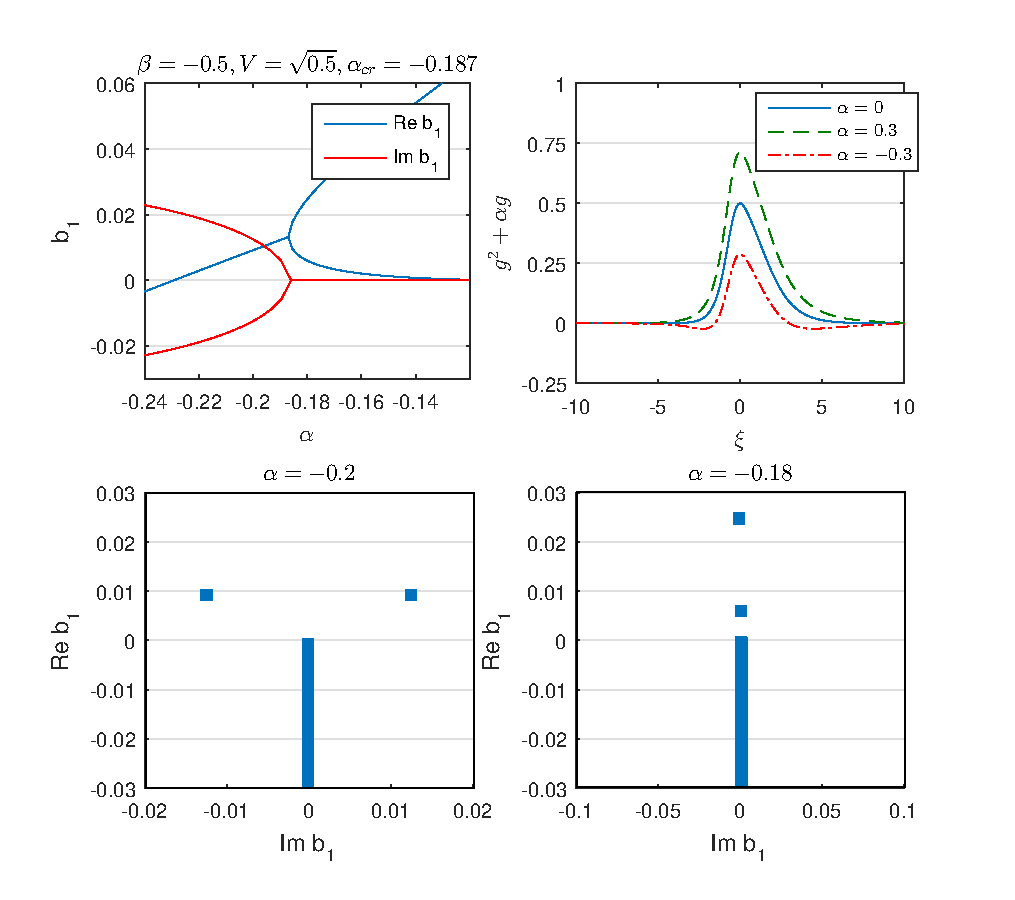
\includegraphics{W_scan_V05_ds-05_insept_b1.eps}}
\end{center}
\caption{Upper left panel shows the eigenvalues of (\ref{lineareqs}) with $V=0.5$, $\beta=-0.5$ as a function of the parameter $\alpha$. Upper right panel shows the effect of the constant $\alpha$ in the shape of the real part of the potential $G$. Lower panels show the eigenvalues  before ($\alpha=-0.18$) and after ($\alpha=-0.2$) the real spectrum breaks into a complex phase. Note the appearance of a complex pair of eigenvalues due to the collision of two real valued eigenvalues at $b=0.013$ where $\alpha_{cr}=-0.187$ (not shown). The spectrum contains an imaginary pair for $\alpha<\alpha_{cr}$.}
\label{fig:FF_phasebreak}
\end{figure}
A phase transition to the complex plane is found for 
$\alpha<\alpha_{cr} = -0.187$,  where a pair of complex 
eigenvalues appear due to the collision of two localized eigenvalues at $b_1=0.013$ (See Fig.\ref{fig:FF_phasebreak}). Note that for $\alpha>0$ there is no phase transition, instead, there is the appearance of additional localized modes due to the higher amplitude of $G$. Here, in contrast with the symmetric system for which $\beta=0$, there are no degenerated discrete eigenvalues as there is no symmetry to induce degeneracy. Instead, as $\alpha$ changes continuously, a complex 
phase may appear only due to the collision of simple discrete 
modes as illustrated in Fig. \ref{fig:FF_phasebreak}. Albeit shown 
here for the specific case of $\beta=-0.5$, different values of 
$\beta$ are found to exhibit the same behavior with respect to 
the breaking of the real valued phase of the spectrum. The effect of different values of the asymmetry constant $\beta$ on the 
eigenvalues $b_1$ is shown in Fig. \ref{fig:beta_spectrum}. In 
subsequent results were considered the values $V=\pm\sqrt{0.5}$. 
Note in (\ref{gform}) that this means that the absolute value of 
the amplitude of $g$ is fixed, only the decay rate of the $\xi>0$ 
region will be allowed to change. This affects the values of 
$b_1$: as $\beta$ decreases, the area of $g$ becomes larger and, consequently,  the number of localized modes increases. Clearly if $\beta=-1$, then
\begin{subequations}
\begin{equation}
\lim_{\xi\to -\infty}G(\xi) =0,
\end{equation}
\begin{equation}
\lim_{\xi\to \infty}G(\xi) =V^2.
\end{equation}
\end{subequations}
\begin{figure}[!htb]
\begin{center}
\scalebox{.55} {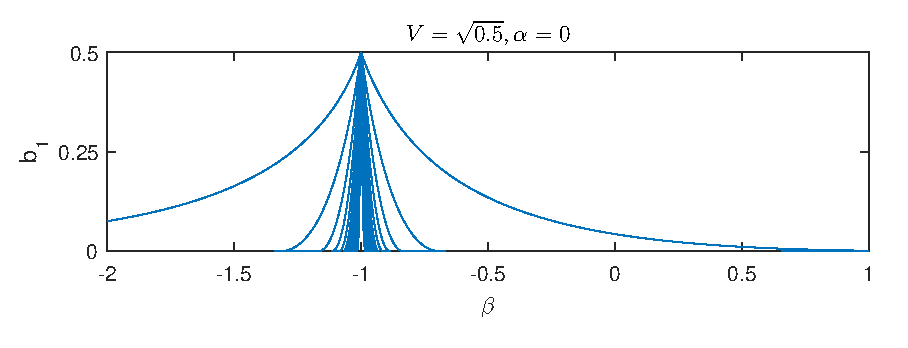
\includegraphics{beta_spectrum.eps}}
\end{center}
\caption{Discrete spectrum of $b_1$ as a function of $\beta$. Note the appearance of a continuous band at $\beta=-1$. The values chosen for the potential are $V=\sqrt{0.5}$ and $\alpha=0$.}
\label{fig:beta_spectrum}
\end{figure}
This is an interesting situation as for $\beta=-1$ the potential $G$ becomes very similar to a Heaviside step function with some localized imaginary part while the spectrum approaches a continuous band defined by $b_1\leq V^2$.
\section{Nonlinear localized modes and linear stability analysis}
Let us now, investigate the existence and stability of the localized solutions of (\ref{stat}). From now on we restrict our considerations mainly to solutions bifurcating from the linear limit, which is understood as a limit defined as $w \to 0$, $b$ tends to a finite eigenmode of the linear problem i.e., $b \to  b_1$. The total energy $P$ of a localized solution is defined by:
\begin{equation}
P=\int_{\infty}^{\infty}\left|w\right|^{2}d\xi.
\end{equation}
Let us now perturb the solution $u(\xi,\zeta)$ by writing:
\begin{equation}
u(\xi,\zeta)=\left(  w(\xi)+p_{+}(\xi)e^{-i\lambda\zeta
}+\overline{p}_{-}(\xi)e^{i\overline{\lambda}\zeta}\right)  e^{ib\zeta
},
\label{smallperturbations}
\end{equation}
 where, $|p_{\pm}(\xi)|\ll 1$, represents small perturbations. Inserting (\ref{smallperturbations}) into (\ref{final}) and collecting linear terms in $p_{\pm}(\xi)$ one  ends up with an eigenvalue problem given by:
\begin{subequations}
\begin{equation}
L_s\left(
\begin{array}
[c]{c}%
p_{2+}\\
p_{-}
\end{array}
\right)  =\lambda\left(
\begin{array}
[c]{c}%
p_{+}\\
p_{-}
\end{array}
\right),
\end{equation}
\begin{equation}
L_s=\left(
\begin{array}
[c]{cc}%
L-b+\sigma\frac{|w|^2(\gamma|w|^2+2)}{(1+\gamma|w|^2)^2}& \sigma\frac{w^2}{(1+\gamma|w|^2)^2} \\
-\sigma\frac{\overline{w}^2}{(1+\gamma|w|^2)^2} &-\overline{L}+b-\sigma\frac{|w|^2(\gamma|w|^2+2)}{(1+\gamma|w|^2)^2}
\end{array}
\right)
\end{equation}
\label{linears}%
\end{subequations}
so that, whenever an eigenvalue $\lambda$ with $\text{Im}(\lambda)>0$ occurs the solution is linearly unstable.

%We have found branches bifurcating from all discrete values of $b$ in the case $V=\pm\sqrt{0.5}$.
\subsection{Effects of saturation parameter $\gamma$}
Investigating the effect of the saturation parameter $\gamma$ we have found that all investigated branches with $\gamma>0$ exhibit a vertical asymptote in the 
$(b,P)$ plane, suppressing the domain of existence of modes, as can be seen in Fig. \ref{fig:gamma_branchesV05sigma1} and Fig. \ref{fig:gamma_branchesV05sigma-1}.
\begin{figure}[!htb]
\begin{center}
\scalebox{.6} {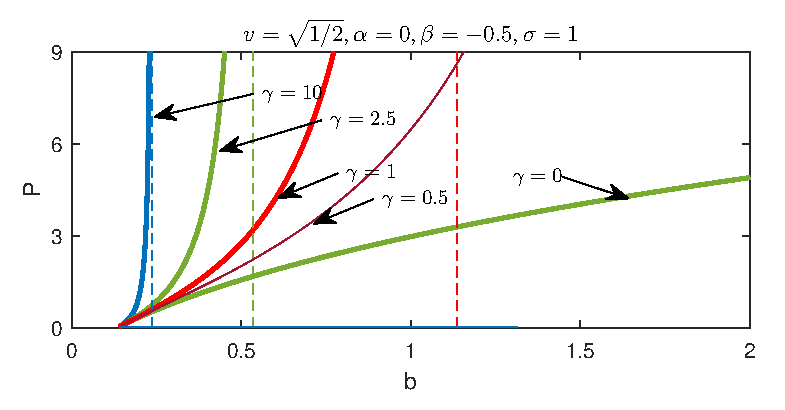
\includegraphics{branches_V05_ds-05_c0_sigma1.eps}}
\end{center}
\caption{Total energy $P$ as a function of $b$ with $V=\sqrt{0.5}$, $\beta=-0.5$, $\sigma=1$ and different values of the saturation constant $\gamma$. Dashed lines represents the asymptotes $b_1+\sigma/\gamma$. Thick lines represent linearly stable solutions and lines represent unstable solutions.}
\label{fig:gamma_branchesV05sigma1}
\end{figure}
\begin{figure}[!htb]
\begin{center}
\scalebox{.67} {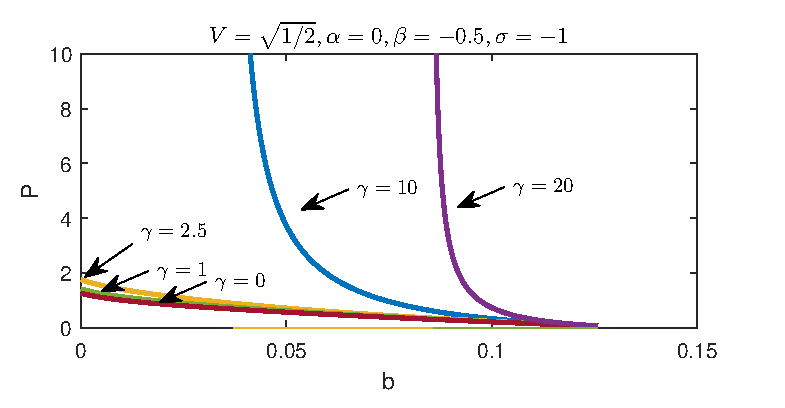
\includegraphics{branches_V05_ds-05_c0_sigma-1.eps}}
\end{center}
\caption{Total energy $P$ as a function of $b$ with $V=\sqrt{0.5}$, $\beta=-0.5$, $\sigma=-1$ and various values of the saturation constant $\gamma$. Thick lines represent linearly stable solutions and lines represent unstable solutions.}
\label{fig:gamma_branchesV05sigma-1}
\end{figure}


This is expected since for solutions with very high intensities one has,
\begin{equation}
\lim_{|w(\xi)|^2\to\infty}{\sigma\frac{|w(\xi)|^2}{1+\gamma|w(\xi)|^2}}=\frac{\sigma}{\gamma}
\label{b_limit}
\end{equation}
Now, inserting (\ref{b_limit}) in (\ref{stat}) we obtain
\begin{equation}
\frac{d^{2}w}{d\xi^{2}}+\left[ g^2+\alpha g+i g_\xi -b+\frac{\sigma}{\gamma}\right]w,
\end{equation}
which, of course the same as (\ref{npt_linear})
\begin{equation}
Lw=(b-\frac{\sigma}{\gamma})w
\end{equation}
and has a localized mode at $b=b_1+\frac{\sigma}{\gamma}$, where $b_1$ is a discrete value of (\ref{npt_linear}). In other words, as the amplitude of the soliton increases its profile becomes similar to the shape of the linear eigenmode it bifurcated in the limit $w\to 0$.
\begin{figure}[!htb]
\begin{center}
\scalebox{.59} {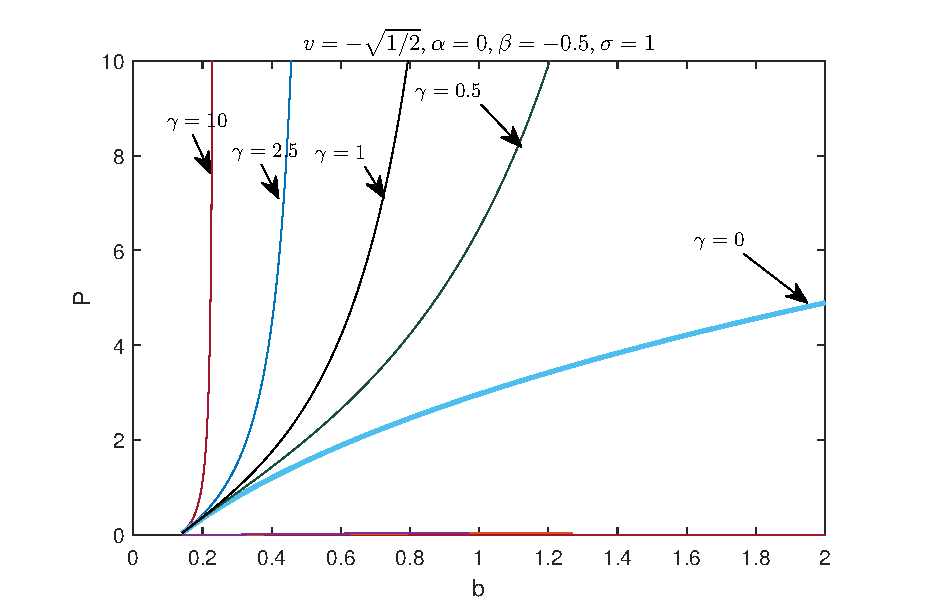
\includegraphics{branches_V-05_ds-05_c0_sigma1_final1.eps}}
\end{center}
\caption{Total energy $P$ as a function of $b$ with $V=-\sqrt{0.5}$, $\beta=-0.5$, $\sigma=1$ and for various values of saturation constant $\gamma$. Right panel shows an expanded view of the region where the transition between stable and unstable solutions occurs. Thick lines represent linearly stable solutions and lines represent unstable solutions.}
\label{fig:gamma_branchesV-05sigma1}
\end{figure}
\begin{figure}[!htb]
\begin{center}
\scalebox{.65} {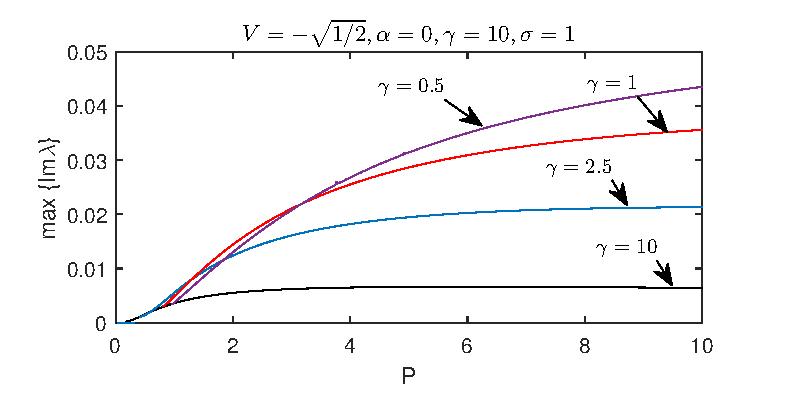
\includegraphics{stab_P_lambda_gamma.eps}}
\end{center}
\caption{Maximum value of imaginary part of (\ref{linears}) as a function of the total energy of localized modes $P$ for several values of $\gamma$. Note that all branches are unstable but $\max \{\text{Im}\lambda\}\to \lambda_{\gamma}$ as $P\to \infty$. The higher the value of $\gamma$, the lower the valuer $\lambda_\gamma$. Parameters are $V=-\sqrt{0.5}$, $\beta=-0.5$, $\sigma=1$.}
\label{fig:stab_P_lambda_gamma}
\end{figure}


\begin{figure}[!htb]
\begin{center}
\scalebox{.65} {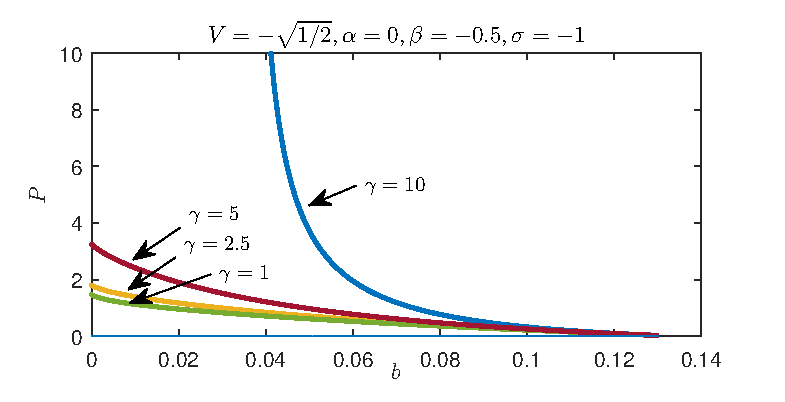
\includegraphics{branches_V-05_ds-05_c0_sigma-1.eps}}
\end{center}
\caption{Total energy $P$ as a function of $b$  with $V=-\sqrt{0.5}$, $\beta=-0.5$, $\sigma=-1$ and different values of saturation constant $\gamma$. All solutions are stable.}
\label{fig:branches_V-05_ds-05_c0_sigma-1}
\end{figure}
In fact, extensive numerical calculations of branches show that the fundamental branches exists in the region $b\in \left(b_1,b_1+\gamma^{-1}\right)$ for the $\sigma=1$ case and $b\in\left(b_1-\gamma^{-1},b_1\right)$ when $\sigma=-1$. Interestingly enough as, using the fact that the branch must be localized within the region between $b_1$ and $b_1+\frac{\sigma}{\gamma}$, one realizes that the $\sigma=1$($\sigma=-1$) branch bifurcates to the right(left). 

In what concerns stability, we have investigated two main potential functions, i.e., $G(\xi)$ and $G^*(\xi)$ which corresponds to the cases $V=\sqrt{0.5}$ and $V=-\sqrt{0.5}$ respectively if one also substitutes $\alpha\to -\alpha$. One can note that if $w$ is a solution of (\ref{stat}) with $G$ then clearly $w^*$ is a solution of (\ref{stat}) with $G^*$. Both solutions clearly have the same $P$. Despite no difference in the $(b,P)-$curve, the stability scenario of the solutions is completely different in each case, as we demonstrate below. First we choose $V=\sqrt{0.5}$. In both cases, $\sigma=\pm 1$,   no linearly unstable solutions were obtained, at least for moderately high amplitude solutions with $P\sim 10$ as is displayed in Fig.\ref{fig:gamma_branchesV05sigma1} and Fig. \ref{fig:gamma_branchesV05sigma-1}. 

With respect to the $V=-\sqrt{0.5}$ case, we have found only unstable solutions in the $\sigma=1$ case as depicted in Fig.  \ref{fig:gamma_branchesV-05sigma1}. The instability here appears due to an asymmetric internal mode that bifurcates from the continuous spectrum of (\ref{linears}), at $\lambda=\pm b$. This internal mode appears as soon as $P>0$, thus there are no stable solutions because this mode moves to the $\text{Im}\lambda>0$ region. Note that this instability rate is quite low when $|b-b_1|\ll 1$. The Fig.  \ref{fig:stab_P_lambda_gamma} clearly shows that branches with higher values of $\gamma$ tend to present a lower degree of instability in this case.  
In the $V=-\sqrt{0.5}$ case we have found stable solutions only in the case of the defocusing nonlinearity, $\sigma=-1$ as is shown in Fig.~\ref{fig:branches_V-05_ds-05_c0_sigma-1}.
\subsection{Effects of asymetry parameter $\beta$}
The effect of different values of the asymmetry constant $\beta$ has also been investigated. We have studied all four combinations of $V=\pm\sqrt{0.5}$ and $\sigma=\pm 1$. See in Fig. \ref{fig:beta_branches_sigma1} and Fig. \ref{fig:branches_V05_sat10_c0_sigma-1} the case $V=\sqrt{0.5}$. The effect of $\beta$ in both $\sigma=\pm 1$ cases is to shift $b_1$ closer to $b_1=0.5$ as expected, with more discrete modes appearing as $\beta\to -1$ (See Fig.~\ref{fig:beta_spectrum}).
\begin{figure}[!htb]
\begin{center}
\scalebox{.6} {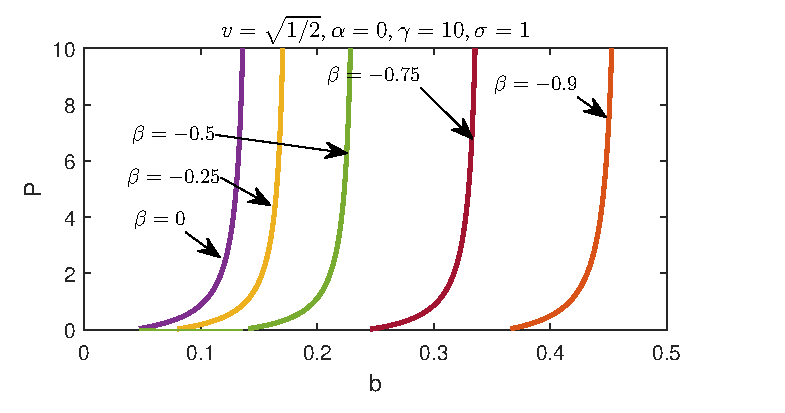
\includegraphics{branches_V05_sat10_c0_sigma1.eps}}
\end{center}
\caption{Total energy $P$ as a function of $b$ with $V=\sqrt{0.5}$, $\beta=-0.5$, $\sigma=1$ and different values of saturation constant $\gamma$. Thick lines (lines) represent linearly stable (unstable) solutions.}
\label{fig:beta_branches_sigma1}
\end{figure}
\begin{figure}[!htb]
\begin{center}
\scalebox{.6} {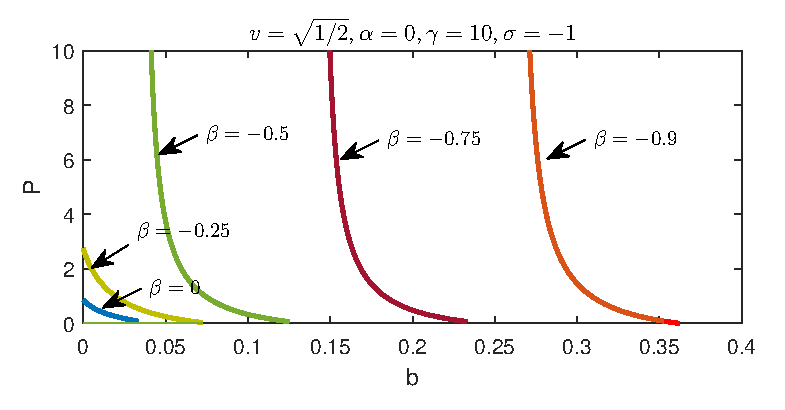
\includegraphics{branches_V05_sat10_c0_sigma-1.eps}}
\end{center}
\caption{Total energy $P$ as a function of $b$  with $V=\sqrt{0.5}$, $\gamma=10$, $\sigma=-1$ and several values of saturation constant $\gamma$. Thick lines (lines) represent linearly stable (unstable) solutions.}
\label{fig:branches_V05_sat10_c0_sigma-1}
\end{figure}
\begin{figure}[!htb]
\begin{center}
\scalebox{.7} {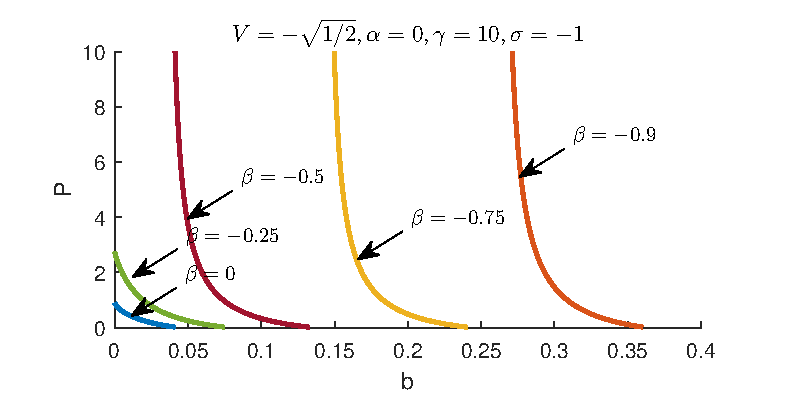
\includegraphics{branches_V-05_sat10_c0_sigma-1.eps}}
\end{center}
\caption{Total energy $P$ as a function of $b$ with $V=-\sqrt{0.5}$, $\gamma=10$, $\sigma=-1$ and various values of asymmetry constant $\beta$. Thick lines (lines) represent linearly stable (unstable) solutions.}
\label{fig:branches_V-05_sat10_c0_sigma-1}
\end{figure}
\begin{figure}[!htb]
\begin{center}
\scalebox{.7} {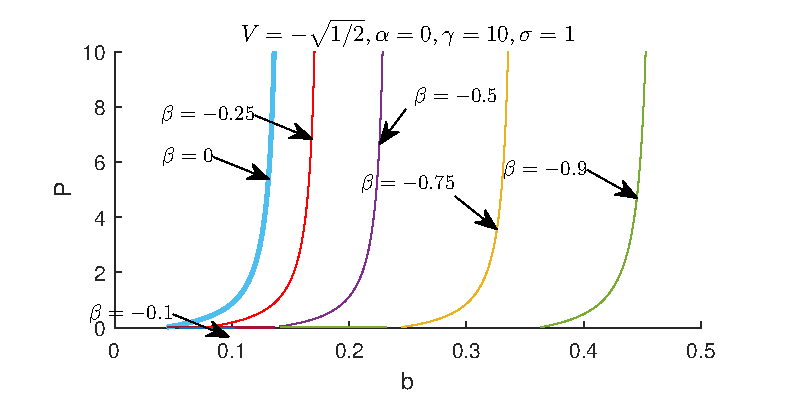
\includegraphics{branches_V-05_sat10_c0_sigma1.eps}}
\end{center}
\caption{Total energy $P$ as a function of $b$ with $V=-\sqrt{0.5}$, $\gamma=10$, $\sigma=1$ and different values of asymmetry  constant $\beta$. Thick lines(lines) represent linearly stable (unstable) solutions.}
\label{fig:branches_V-05_sat10_c0_sigma1}
\end{figure}
The vertical asymptote $b=b_1+\sigma/\gamma$ is still present in the branches. Regarding stability, no changes were observed: all solutions were found to be stable in the $V=\sqrt{0.5}$ case as illustrated in Fig.~\ref{fig:beta_branches_sigma1} and Fig.~\ref{fig:branches_V05_sat10_c0_sigma-1}. Solutions with $V=-\sqrt{0.5}$ are stable for $\sigma=-1$ (See Fig.~\ref{fig:branches_V-05_sat10_c0_sigma-1}) and  all solutions are unstable in the $\sigma=1$ case (See Fig.~\ref{fig:branches_V-05_sat10_c0_sigma1}). 

\begin{figure}[!htb]
\begin{center}
\scalebox{.7} {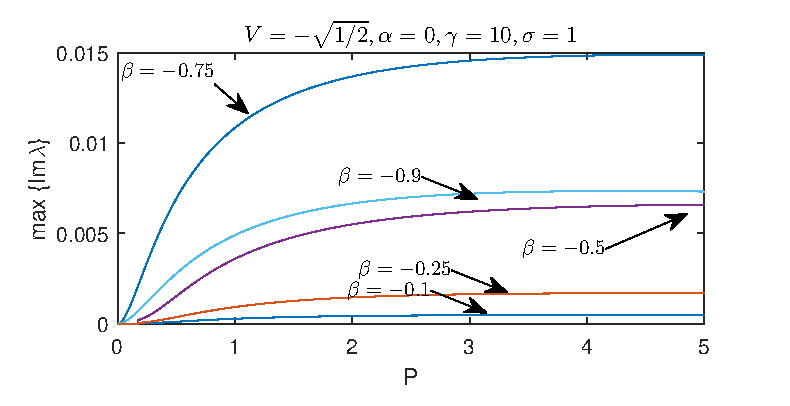
\includegraphics{stab_P_lambda.eps}}
\end{center}
\caption{Maximum value of the imaginary part of (\ref{linears}) as a function of total energy of localized modes $P$. Note that all 
$\beta<0$ branches are unstable but $\max \{\text{Im}\lambda\}\to 0$ as $\beta\to 0$. Parameters are $V=-\sqrt{0.5}$, $\gamma=10$, 
$\sigma=1$.}
\label{fig:stab_P_lambda}
\end{figure}
Note that in both $\sigma=\pm 1$ cases with $V=-\sqrt{0.5}$ there are stable solutions only if $\beta=0$, i.e., the $\PT$-symmetric case. In Fig. \ref{fig:stab_P_lambda} we can see that in fact $\max \{\text{Im}\lambda\}\to 0$ as $\beta\to 0$.


\subsection{Investigation of gain and loss parameter $\alpha$}
		Here we fix $\beta=-0.5$, $\gamma=10$ and change $\alpha$ to investigate its effects on the existence and stability of fundamental branches. The first case to be investigated is the one with $V=\sqrt{0.5}$ and $\sigma=1$ and we turn to Fig.~\ref{fig:branches_V05_sat10_ds-05_sigma1}, from where one may conclude that all observed solutions are stable. The second case with $V=\sqrt{0.5}$ and $\sigma=-1$ shows that an unstable region may exist above some threshold in $P$ if $\alpha<0$ is close enough to $\alpha_{cr}$. The stable region becomes smaller as $\alpha$ gets closer to $\alpha_{cr}$, eventually disappearing along with the branch itself when $\alpha\to\alpha_{cr}$. Next, in the $V=-\sqrt{0.5}$ and $\sigma=1$ case we note that there are no stable solutions. Finally, in the $V=-\sqrt{0.5}$ and $\sigma=-1$, all solutions are stable.
\begin{figure}[!htb]
\begin{center}
\scalebox{.7} {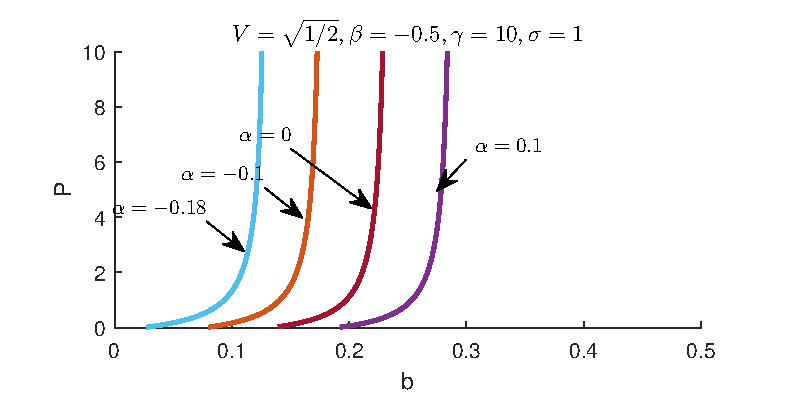
\includegraphics{branches_V05_sat10_ds-05_sigma1.eps}}
\end{center}
\caption{Total energy $P$ as a function of $b$ with $V=\sqrt{0.5}$, $\gamma=10$, $\sigma=1$ and various values of $\alpha$. Thick lines (lines) represent linearly stable (unstable) solutions.}
\label{fig:branches_V05_sat10_ds-05_sigma1}
\end{figure}
\begin{figure}[!htb]
\begin{center}
\scalebox{.7} {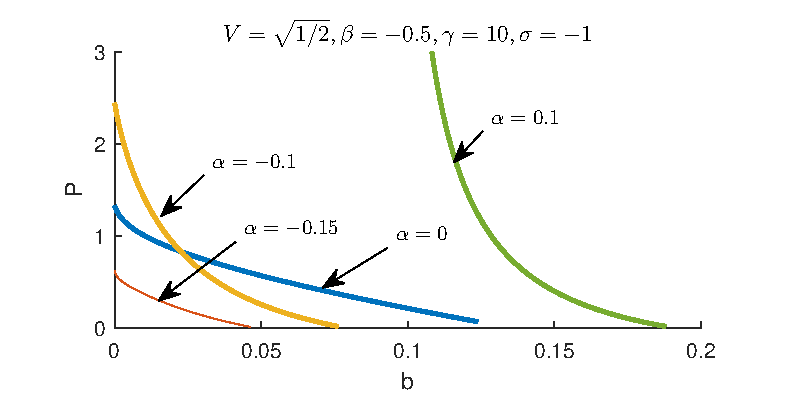
\includegraphics{branches_V05_sat10_ds-05_sigma-1.eps}}
\end{center}
\caption{Total energy $P$ as a function of $b$  with $V=\sqrt{0.5}$, $\gamma=10$, $\sigma=-1$ and several  values of $\alpha$. Thick lines (lines) represent linearly stable (unstable) solutions.}
\label{fig:branches_V05_sat10_ds-05_sigma-1}
\end{figure}

\begin{figure}[!htb]
\begin{center}
\scalebox{.7} {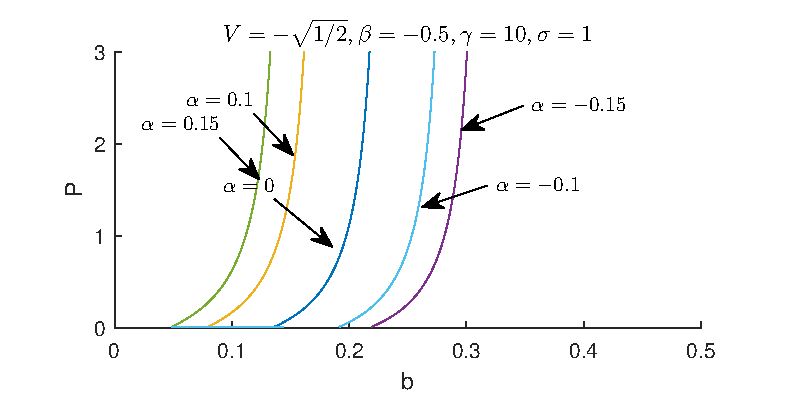
\includegraphics{branches_V-05_sat10_ds-05_sigma1.eps}}
\end{center}
\caption{Total energy $P$ as a function of $b$ with $V=-\sqrt{0.5}$, $\gamma=10$, $\sigma=1$ and different values of $\alpha$. Thick lines (lines) represent linearly stable (unstable) solutions.}
\label{fig:branches_V-05_sat10_ds-05_sigma1}
\end{figure}

\begin{figure}[!htb]
\begin{center}
\scalebox{.7} {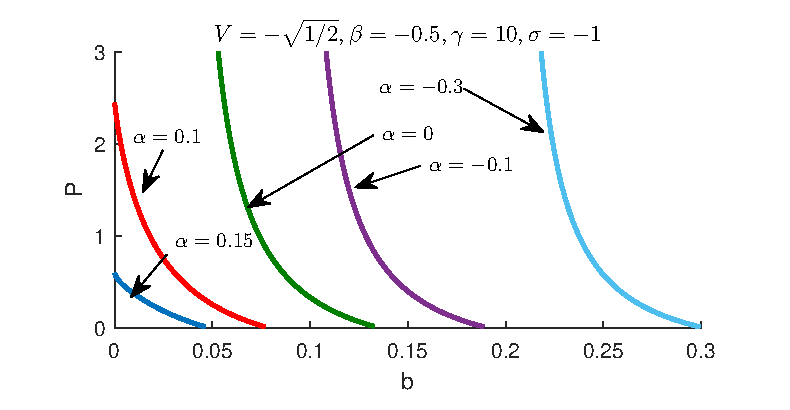
\includegraphics{branches_V-05_sat10_ds-05_sigma-1_final.eps}}
\end{center}
\caption{Total energy $P$ as a function of $b$ with $V=-\sqrt{0.5}$, $\gamma=10$, $\sigma=1$ and different values of asymmetry  constant $\beta$. Thick lines (lines) represent linearly stable (unstable) solutions.}
\label{fig:branches_V-05_sat10_ds-05_sigma-1}
\end{figure}




\section{Dynamics of localized solutions}

To corroborate the results described in the last section, in this section we proceed  to make comparisons between the model of perturbations (\ref{linears}) and direct propagation of (\ref{stat}) using the solutions found as initial conditions in (\ref{final}). In all propagations we have added a $1\%$ of noise to the amplitude at $\zeta=0$. Here our objective is to show that the linear stability analysis predicts quite well the evolution of localized modes under weak perturbations.
\begin{figure}[ht]
\begin{center}
\scalebox{.75} {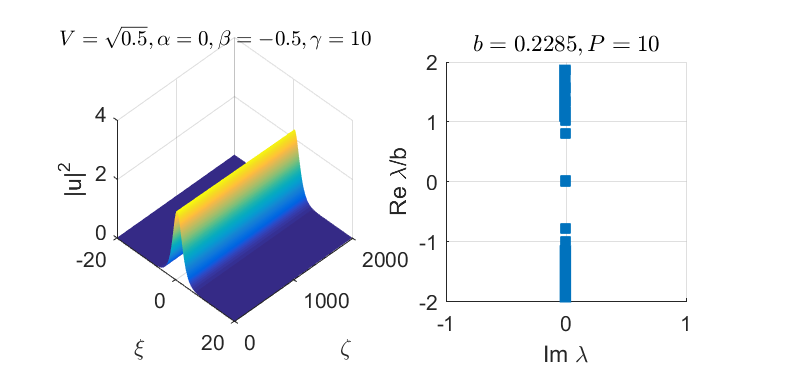
\includegraphics{prop_V05_sat10_ds-05_c0_sigma1_highpower.eps}}
\end{center}
\caption{(Color online)(Left panel) Intensity $|u|^2$ during propagation of a high power $P=10$ stable soliton with $b=0.23$. (Right panel) Corresponding eigenvalues of (\ref{linears}). Parameters are $V=\sqrt{0.5},\beta=-0.5,\alpha=0,\gamma=10$ and $\sigma=1$.}%
\label{fig:prop_V05_sat10_ds-05_c0_sigma1_highpower}%
\end{figure}
\begin{figure}[ht]
\begin{center}
\scalebox{.83} {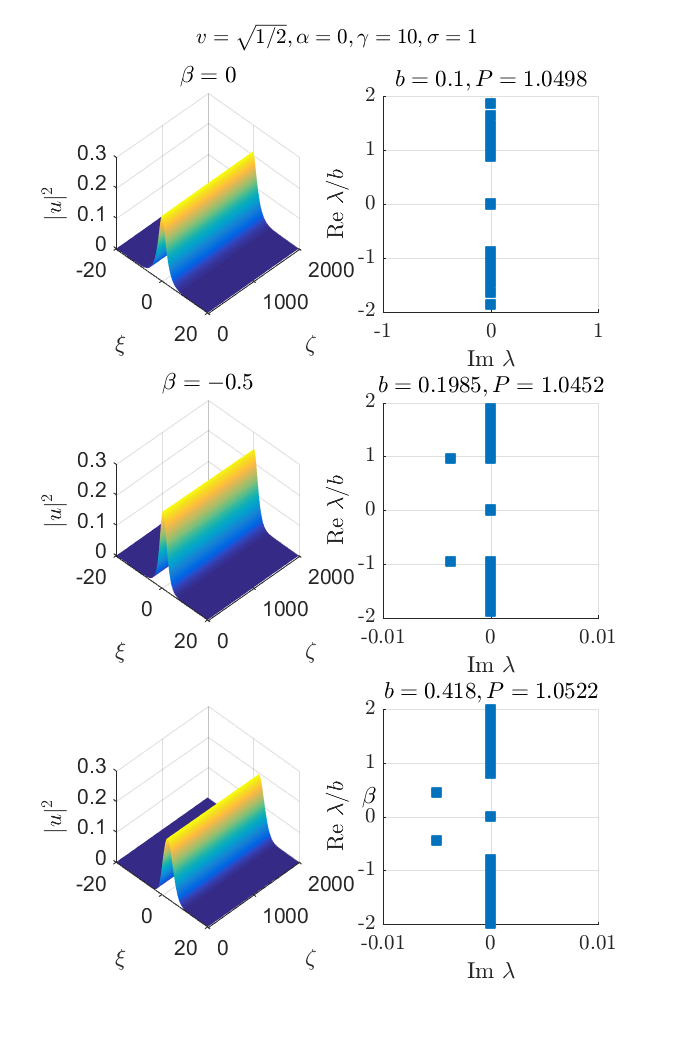
\includegraphics{prop_beta_sigma1.eps}}
\end{center}
\caption{(Color online)(Left panels) Intensities $|u|^2$ during propagation of stable solutions of branches with different values of assymetry constant $\beta$. Parameters are $V=\sqrt{0.5},\alpha=0,\gamma=10$ and $\sigma=1$.}%
\label{fig:prop_beta_sigma1}%
\end{figure}
\begin{figure}[ht]
\begin{center}
\scalebox{.68} {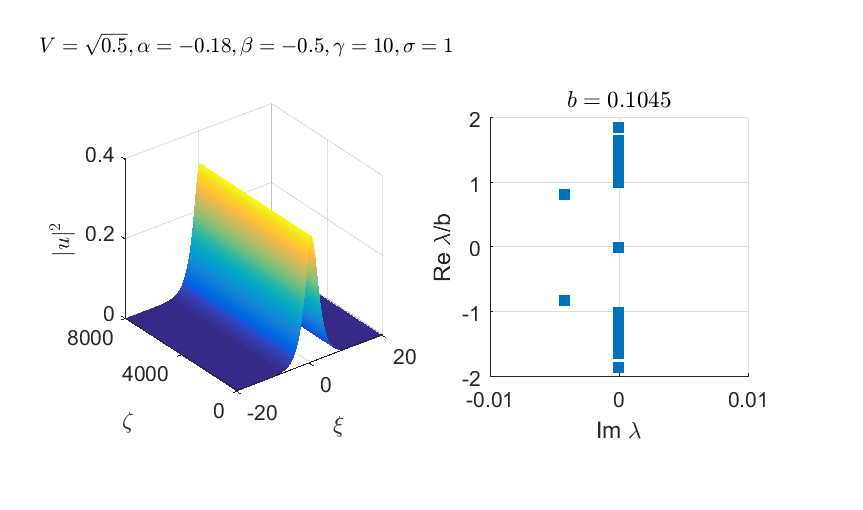
\includegraphics{prop_V05_sat10_ds-05_c-018_sigma1.eps}}
\end{center}
\caption{(Color online)(Left panels) Intensity $|u|^2$ during propagation of a stable solution with $b=0.1$. Parameters are $V=\sqrt{0.5},\beta=-0.5,\alpha=-0.18,\gamma=10$ and $\sigma=1$.}%
\label{fig:prop_V05_sat10_ds-05_c-018_sigma1}%
\end{figure}
The first property that we have observed is the stability of  three among four possible combinations of signals of $V$ and $\sigma$, three cases: $V=\sqrt{0.5}$ and $\sigma=\pm1$;$V=-\sqrt{0.5}$ and $\sigma=-1$, exhibit stable solutions as possible to see in Fig.~\ref{fig:prop_V05_sat10_ds-05_c0_sigma1_highpower}, Fig.~\ref{fig:prop_beta_sigma1} and Fig.~\ref{fig:prop_V05_sat10_ds-05_c-018_sigma1} for the $V=\sqrt{0.5}$ and $\sigma=1$ case. In all figures of dynamics we used $\gamma=10$ as it does not change the existence or absence of stable solutions. Note that discrete modes of stable solitons with $\beta\neq 0$ go into the negative imaginary part plane, differently from the $\beta=0$ case, where discrete modes of stable solitons must have $\text{Im}\lambda=0$ as possible to see in Fig.~\ref{fig:prop_beta_sigma1} . In Fig. \ref{fig:prop_V05_sat10_ds-05_c-018_sigma1} we show the evolution of a stable solution with $\alpha=-0.18$, close but below the phase transition of the real spectrum. 

An example of the dynamics of an unstable solution for the case $V=\sqrt{0.5}$, $\gamma=10$ and $\sigma=-1$ is shown in Fig.~\ref{fig:prop_V05_sat10_ds-09_c0_sigma-1} for the $\alpha=0$ case with $\beta=-0.9$. In Fig.~\ref{fig:prop_V05_sat10_ds-05_c-014_sigma-1} we show two examples of unstable solutions  in the branch with $\alpha=-0.14$ $\beta=-0.5$. Note that while $\beta$ does not change by itself the stability properties of the solutions when all other parameters are fixed, the parameter $\alpha<0$ may in fact introduce instability in the system, both of oscillatory (complex $\lambda$) and purely exponentially decaying (purely complex $\lambda$) types, as displayed in Fig.~\ref{fig:prop_V05_sat10_ds-05_c-014_sigma-1}.
\begin{comment}
\begin{figure}[ht]
\begin{center}
\scalebox{.85} {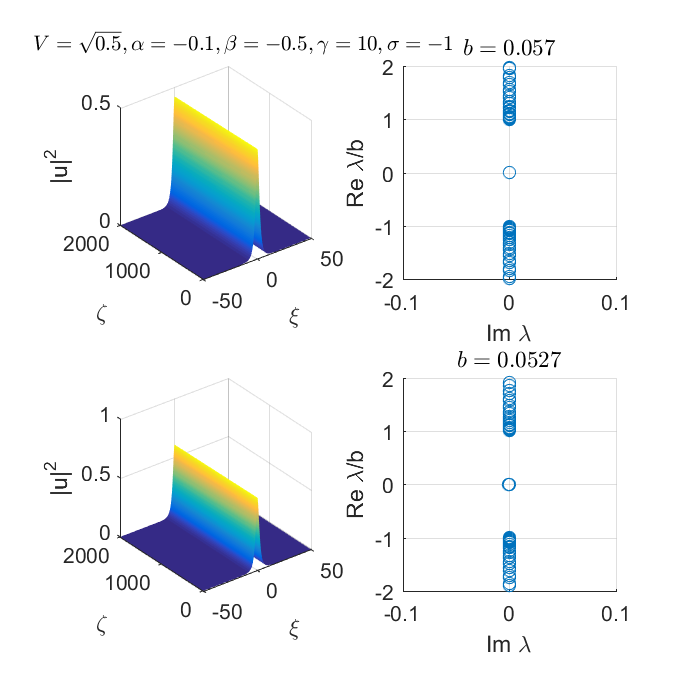
\includegraphics{prop_V05_sat10_ds-05_c-01_sigma-1.eps}}
\end{center}
\caption{(Color online)(Left panels) Intensities $|u|^2$ during propagation of stable solutions. (Right panels) Corresponding eigenvalues of (\ref{linears}) Note the that de linear stability model correctly predicts the onset of a oscillatory instability in the solution with $b=0.0153$. Parameters are $V=\sqrt{0.5},\alpha=-0.1,\beta=-0.5,\gamma=10$ and $\sigma=-1$.}%
\label{fig:prop_V05_sat10_ds-05_c-01_sigma-1}%
\end{figure}
\end{comment}
\begin{figure}[ht]
\begin{center}
\scalebox{.73} {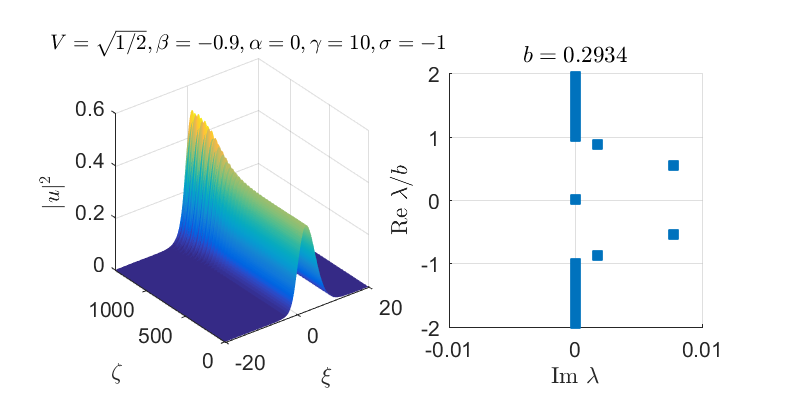
\includegraphics{prop_V05_sat10_ds-09_c0_sigma-1.eps}}
\end{center}
\caption{(Color online)(Left panel) Intensity $|u|^2$ during propagation for an unstable solution. Parameters are $V=\sqrt{0.5},\beta=-0.9,\alpha=0,\gamma=10$ and $\sigma=-1$.}%
\label{fig:prop_V05_sat10_ds-09_c0_sigma-1}%
\end{figure}
\begin{figure}[ht]
\begin{center}
\scalebox{.75} {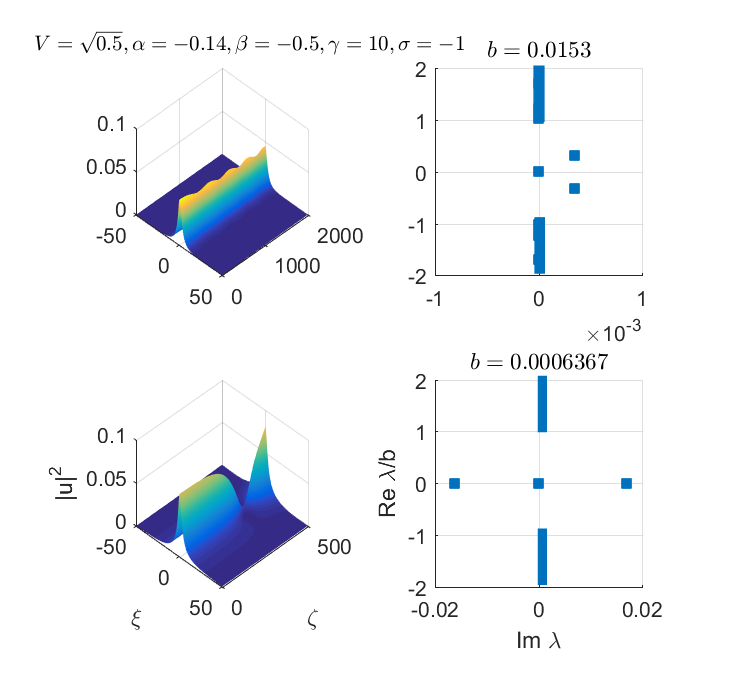
\includegraphics{prop_V05_sat10_ds-05_c-014_sigma-1.eps}}
\end{center}
\caption{(Color online)(Left panels) A Intensities $|u|^2$ during propagation of unstable solutions. (Right panels) Corresponding eigenvalues of (\ref{linears}) Note the that de linear stability model correctly predicts the onset of a oscillatory instability in the solution with $b=0.0153$ and the exponential decay in the case $b=0.0006367$. Parameters are $V=\sqrt{0.5},\beta=-0.5,\alpha=-0.14,\gamma=10$ and $\sigma=-1$.}%
\label{fig:prop_V05_sat10_ds-05_c-014_sigma-1}%
\end{figure}

Dynamics of propagation in case $V=-\sqrt{0.5}$ and $\sigma=1$ are shown in both cases, i.e., unstable (Fig.\ref{fig:prop_V-05_sat10_ds-05_c0_sigma1} ) and  stable (Fig.\ref{fig:prop_V-05_sat10_ds-05_c0_sigma-1_final}).
\begin{figure}[ht]
\begin{center}
%\scalebox{.75} {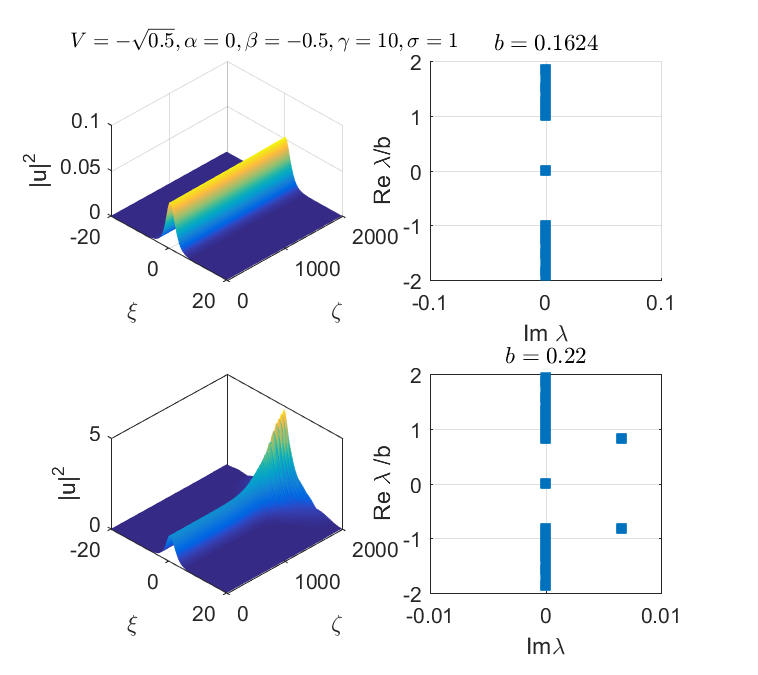
\includegraphics{prop_V-05_sat10_ds-05_c0_sigma1.eps}}
\scalebox{.75} {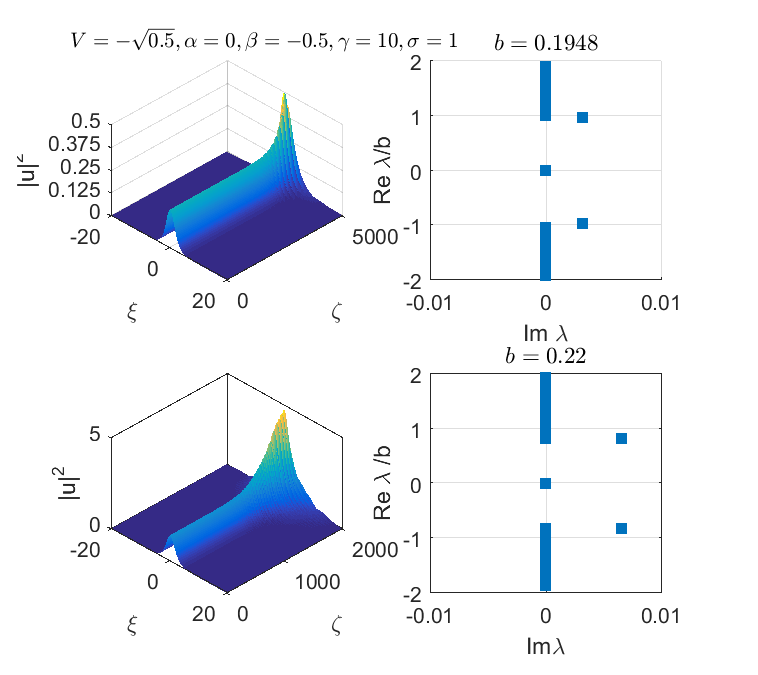
\includegraphics{prop_V-05_sat10_ds-05_c0_sigma1_final.eps}}
\end{center}
\caption{(Color online)(Left panels) Intensities $|u|^2$ during propagation for unstable solutions. (Right panels) Corresponding eigenvalues of (\ref{linears}). Note the that de linear stability model correctly predicts the onset of a oscillatory instability. Also note that the instability develops quite slowly. Parameters are $V=-\sqrt{0.5},\beta=-0.5,\alpha=0,\gamma=10$ and $\sigma=1$.}%
\label{fig:prop_V-05_sat10_ds-05_c0_sigma1}%
\end{figure}
Finally in Fig.\ref{fig:prop_V-05_sat10_ds-05_c0_sigma-1} we show the dynamics of a stable solution in the case $V=-\sqrt{0.5}$ and $\sigma=-1$.
\begin{figure}[ht]
\begin{center}
\scalebox{.73} {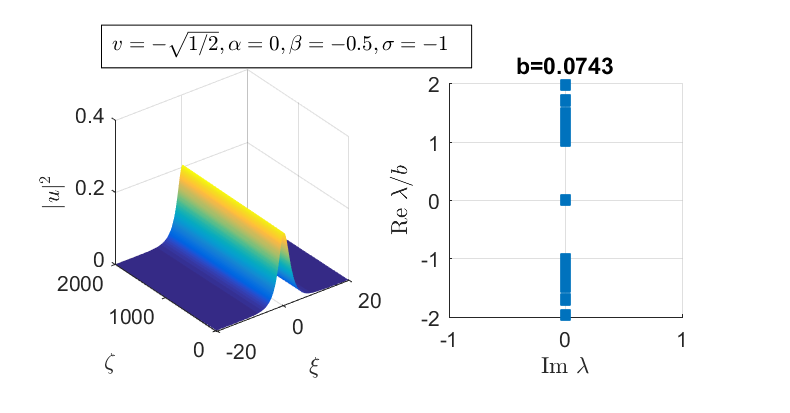
\includegraphics{prop_V-05_sat10_ds-05_c0_sigma-1.eps}}
\end{center}
\caption{(Color online)(Left panel) Intensity $|u|^2$ during propagation for a stable solution. Parameters are $V=-\sqrt{0.5},\beta=-0.5,\alpha=0,\gamma=10$ and $\sigma=-1$.}%
\label{fig:prop_V-05_sat10_ds-05_c0_sigma-1}%
\end{figure}

\begin{figure}[ht]
\begin{center}
\scalebox{.73} {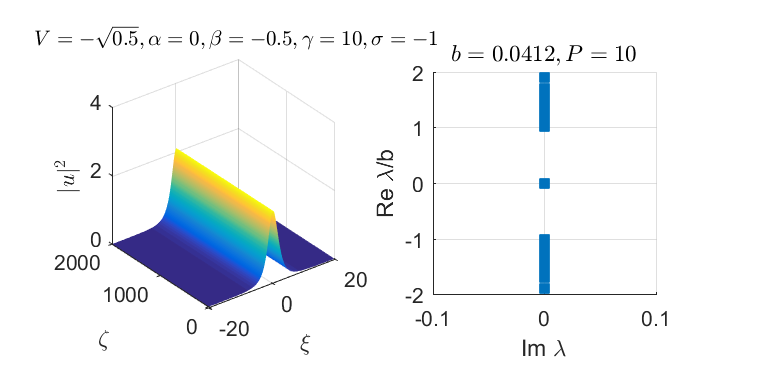
\includegraphics{prop_V-05_sat10_ds-05_c0_sigma-1_final.eps}}
\end{center}
\caption{(Color online)(Left panel) Intensity $|u|^2$ during propagation for a high power, $P=10$, stable solution with $b=0.0412$. Parameters are $V=-\sqrt{0.5},\beta=-0.5,\alpha=0,\gamma=10$ and $\sigma=-1$.}%
\label{fig:prop_V-05_sat10_ds-05_c0_sigma-1_final}%
\end{figure}

Looking at the stability spectrum of (\ref{linears}) we can see that the role of the sign of $V$ has in respect to stability of branches can be explained: First we see that non-$\PT$-symmetric cases, i.e., $\beta\neq 0$, do not possess the symmetry $\lambda=\lambda^*$ as expected. So one can have discrete eigenvalues $\lambda$ in either $\text{Im}\lambda>0$ or $\text{Im}\lambda<0$ regions. Now, if one investigate a branch where the potential is substituted for $G\to G^*$ the spectrum of (\ref{linears}) changes to $\lambda\to\lambda^*$ as all terms other terms other than $L$ are real in $L_s$. So whenever an stable solution exists with some $\text{Im}\lambda<0$ for a given $G$ there is a unstable solution in the branch of the system with the potential $G^*$. There are cases where changing $G$ for $G^*$ does not change the stability of a function. This happens when a stable solution only has $\text{Im}\lambda=0$ as possible to see in Fig. \ref{fig:prop_V05_sat10_ds-05_c0_sigma1_highpower} and Fig~\ref{fig:prop_V-05_sat10_ds-05_c0_sigma-1_final} for examples.

%\begin{figure}[ht]
%\begin{center}
%\scalebox{.63} {\includegraphics{prop_V05_ds-05c0_FF.eps}}
%\end{center}
%\caption{(Color online)(Left panels) Intensities $|u_{1}|^2$ during propagation for stable( upper and lower panels) and an unstable (middle panel). (Right panels) Corresponding eigenvalues of (\ref{linears}) Note the that de linear stability model correctly predicts the onset of a oscillatory instability in the solution with $b=0.14$. All solutions pertain to the $b$ branch. Parameters are $\alpha=0$ and $\beta=-0.5$}%
%\label{fig:prop_V05_ds-05c0_FF}%
%\end{figure}

\section{Conclusions}

In conclusion, we have studied the existence and stability properties of soliton  families in media with a saturable nonlinearity embedded in a non-$\PT$-symmetric complex refractive index. We 
have found the that such media does support the existence of asymmetric solitons in both self-focusing as well self-defocusing case. Furthermore, 
all branches of solitons found to bifurcate from the linear limit in case the saturation parameter $\gamma \neq 0$, exhibit a vertical asymptote in the power-eigenvalue diagram, revealing that $\gamma$ restricts severely
the range where localized modes that are supported, in comparison 
with a Kerr nonlinearity where there is no restriction. Also, the $b$ asymptotic value for large powers is uniquely determined by the saturation 
parameter, and larger saturation parameters lead to greater reduction in 
the mode range. This result is similar to the result reported in ${\cal PT}$- optical lattices \cite{Hu-Hu}. Furthermore, as the amplitude of the soliton increases its profile becomes similar to the shape of the linear eigenmode from where it was originated. In case of positive $V$ we find stable solitons in both media, i.e.,  under the effect of self-focusing or self-defocusing. In cases where $V$ assumes negative values we find that, as the amplitude of the soliton depends on $V^2$ nothing changes in the spectrum. However, when it comes to the stability properties these are complete altered and all solutions become unstable in the 
self-focusing media, i. e. for $\sigma = 1$. Variations on the value of $\alpha$ do not change the overall  picture, except for the locations where the nonlinear modes are created. All the analytic results have been 
confronted with numerical simulations displaying the propagation of 
stable and unstable nonlinear modes with a remarkable agreement. 
We hope that our investigation on waveguides, combining saturable nonlinearity and asymmetric complex potentials reveals itself to be 
useful for applications
in optics widening the class of metamaterials that may be tailored
to control light propagation in waveguides and thus, providing novel techniques. 


\acknowledgments
The authors grateful acknowledge the partial financial support from the Brazilian agencies, CNPq and Capes. 
\begin{thebibliography}{99}

\bibitem{Bender1}
C. M. Bender and S. Boettcher, Phys.Rev.Lett. {\bf 80}, 5243 (1998);%A. Mostafazadeh   %Pseudo-Hermiticity for a class of nondiagonalizable Hamiltonians. Journal of Mathematical Physics,
%{\bf 43}, 6343 (2002)

\bibitem{Ruter2010} C. E. Ruter, K. G. Makris, R. El-Ganainy, D. N. Christodoulides, M. Segev, and D. Kip, Nat. Phys. {\bf 6}, 192 (2010).

\bibitem{peschel}  A. Regensburger, C. Bersch, M. A. Miri, G. Onishchukov, D. N. Christodoulides, and U. Peschel, Nature (London) {\bf 488}, 167
(2012).

\bibitem{peng} B. Peng, S. O ̈zdemir, F. Lei, F. Monifi, M. Gian- freda, G. Long, S. Fan, F. Nori, C.M. Bender, and L. Yang, Nat. Phys. {\bf10}, 394 (2014).

\bibitem{Guo} A. Guo, G. J. Salamo, D. Duchesne, R. Morandotti, M. Volatier-Ravat, V. Aimez, G. A. Siviloglou and D. N.
Christodoulides Phys. Rev. Lett. {\bf103}, 093902 (2009). 

\bibitem{Longhi} S. Longhi, Phys. Rev. Lett. {\bf105}, 013903 (2010).

\bibitem{Makris} K. G. Makris, R. El-Ganainy, D. N. Christodoulides, and Z. H. Musslimani, Phys. Rev. Lett. 100, 103904 (2008).

\bibitem{feng2013} L. Feng, Y.L. Xu, W.S. Fegadolli, M.H. Lu, J.E.B. Oliveira, V.R. Almeida, Y.F. Chen, 
and A. Scherer,Nature Materials {\bf12}, 108 (2013).

\bibitem{feng2014} L. Feng, Z.J. Wong, R. Ma, Y. Wang, and X. Zhang, Science {\bf346}, 972 (2014).

\bibitem{science14} H. Hodaei, M.A. Miri, M. Heinrich, D. N. Christodoulides, and M. Khajavikhan, Science {\bf346}, 975 (2014).


\bibitem{Christodoulides1} Z. H. Musslimani, K. G. Makris, R. El-Ganainy, and D. N. Christodoulides
Phys. Rev. Lett. {\bf 100}, 030402, (2008).

\bibitem{malomed11} R. Driben and B. A. Malomed, Opt. Lett. {\bf36}, 4323 (2011).

\bibitem{konotop12} D. A. Zezyulin and V.V. Konotop, Phys. Rev. A {\bf85}, 043840 (2012).

\bibitem{yang12} S. Nixon, Y. Zhu and J. Yang, Opt. Lett. {\bf37}, 4874 (2012).

\bibitem{segev13} Y. Lumer, Y. Plotnik, M. C. Rechtsman, and M. Segev, Phys. Rev. Lett. {\bf111}, 263901 (2013).

\bibitem{ulf15} M. Wimmer, A. Regensburger, M. Miri, C. Bersch, D. N. Christodoulides and U. Peschel, Nature Comm. {\bf6} 7782 (2015).


\bibitem{Cannata1998} F. Cannata, G. Junker, and J. Trost, Phys. Lett. A {\bf 246},219–226 (1998).
\bibitem{Miri2013} M.A. Miri, M. Heinrich, and D. N. Christodoulides, Phys. Rev. A {\bf 87}, 043819 (2013).
\bibitem{Tsoy2014} E.N. Tsoy, I.M. Allayarov and F. Kh. Abdullaev, Opt. Lett. {\bf 39}, 4215–4218 (2014).
\bibitem{Yang2016} S. Nixon and J. Yang, Phys. Rev. A {\bf 93}(3), 031802 (2016).
\bibitem{npt_solitons} E. N. Tsoy, I. M. Allayarov, and F. Kh. Abdullaev, Opt. Lett.
\bibitem{moreira16} F. C. Moreira and S. B. Cavalcanti, Phys. Rev. A {\bf 94}, 043818.
\bibitem{gatz} S. Gatz and J. Herrmann, J. Opt. Soc. Am. B {\bf 8}, 2296-2302 (1991)  
\bibitem{Segev} M. Segev, B. Crosignani, A. Yariv and B. Fischer, Phys. Rev. Lett. {\bf 68}, 923 (1992).

\bibitem{Znojil}
M. Znojil, J.Phys. A Math. Gen. {\bf 33},  L61 (2000).


\bibitem{Ahmed}
%Z. Ahmed, Phys.Lett. A {\bf 282}, 343 (2001).
Z. Ahmed, Phys. Lett. A {\bf 282}, 343-348 (2001).

\bibitem{Gaussian} S. Hu, Xuekai Ma, Daquan Lu, Zhenjun Yang, Yizhou Zheng, and Wei Hu    %Solitons supported by complex $\PT$--symmetric Gaussian potentials.
Phys. Rev. A, {\bf 84}, 043818  (2011).


\bibitem{defoc} Zhiwei Shi, Xiujuan Jiang, Xing Zhu, and Huagang Li, Phys. Rev. A {\bf 84}, 053855 (2011)

\bibitem{AKOS} F. K. Abdullaev, V. V. Konotop, M. \"Ogren, and M. P. S\o rensen,
%Zeno effect and switching of solitons in nonlinear couplers.
Opt. Lett., {\bf 36}, 4566 (2011).

\bibitem{double_well} H. Cartarius and G. Wunner  arXiv:1203.1885v1 (2012).

\bibitem{Moreira_loc} F. C. Moreira, F. Kh. Abdullaev, V. V. Konotop, and A. V. Yulin, Phys. Rev. A {\bf 86}, 053815 (2012).











\textbf{39}, 4215 (2014); V. V. Konotop and D. A. Zezyulin, Opt. Lett. \textbf{39}, 5535 (2014).









\bibitem{Hu-Hu} S. Hu and Wei Hu, Physica B {\bf 429}, 28 (2013).

\begin{comment}
\bibitem{Muga}
A. Ruschaupt, F. Delgado and J. G. Muga, J. Phys. A {\bf 38} L171 (2005).

\bibitem{Exp1}
A. Guo, G. J. Salamo, D.Duchesne,R. Morandotti, M. Volatier-Ravat, V. Aimez, G.A. Siviloglou, D.N. Christodoulides,
Phys. Rev. Lett., {\bf 103}, 093902 (2009); C. E. R\"uter, K.G.Makris, R. El-Ganainy,D.N. Christodoulides, M. Segev, and D. Kip, Nat. Phys. 6, 192 (2010).




\bibitem{Mostafa_scattering} A. Mostafazadeh,
%Resonance phenomenon related to spectral singularities, complex barrier potential, and resonating %waveguides.
Phys. Rev. A, {\bf 80} 032711 (2009).

\bibitem{Kottos} O. Bendix, R. Fleischmann, T. Kottos, and B. Shapiro,
%Exponentially Fragile $\PT$- Symmetry in Lattices with Localized Eigenmodes.
Phys. Rev. Lett. {\bf 103},  (2009)






\bibitem{PT-_sol}
F. Kh. Abdullaev, V.V. Konotop, M. Salerno, and A. V. Yulin, Phys. Rev. E {\bf 82}, 056606 (2010);
F. Kh. Abdullaev, Y. V. Kartashov, V.V. Konotop, and D. A. Zezyulin, Phys. Rev. A {\bf 83}, 041805(R) (2011);
Y. He , X. Zhu, D. Mihalache, J. Liu and Z. Chen, Phys. Rev. A {\bf 85}, 013831 (2012);
S. Nixon, L. Ge, and J.Yang, Phys. Rev A {\bf 85}, 023822 (2012);
V. Achilleos, P. G. Kevrekidis,  D. J. Frantzeskakis, and R. Carretero-Gonzales,  Phys. Rev. A {\bf 86 }, 013808  (2012);
J. Zeng and Y. Lan, Phys.Rev. E {\bf 85}, 047601 (2012); S.V. Suchkov, S.V. Dmitriev, B. A. Malomed, and Yu. S. Kivshar, Phys. Rev. A {\bf 85}, 033825 (2012).

%\bibitem{Suchkov}
%S. Suchkov et al. Phys. Rev. A {\bf 85}, 033825 (2012).

\bibitem{Clausen1}
 C.B. Clausen, J.P. Torres, and L. Torner, Phys. Lett. A {\bf 249}, 455 (1998).

\bibitem{Clausen2}
C.B. Clausen and L. Torner, Phys. Rev. Lett. {\bf 81}, 790 (1998).




%\bibitem{Moreira_per} F. C. Moreira, V. V. Konotop, and B. A. Malomed, Phys. Rev. A {\bf 87}, 013832 (2013).







\bibitem{Ahmmed2001} Z. Ahmed, Phys. Lett. A {\bf 282}, 343 (2001)



\bibitem{Yang2015}S. Nixon and J. Yang, Phys. arXiv \textit{preprint} arXiv:1509.07057 (2015).

Phys. Rev. A 93, 031802(R) – Published 9 March 2016 All-real spectra in optical systems with arbitrary gain and loss distributions

\bibitem{Midya}
B. Midya, B. Roy, R. Roychoudhury, Phys. Lett. A {\bf 374} 2605-2607 (2010).

\bibitem{Landau}
D. Landau, E. M. Lifshitz, \textit{Quantum Mechanics: Non-Relativistic Theory, Volume {\bf 3}}, (Elsevier Science, MA, 1958)

\bibitem{Zezyulin}
D. A. Zezyulin and V.V. Konotop, Phys. Rev. Lett. {\bf 108}, 213906 (2012).

\bibitem{Tsoy}
E.N. Tsoy, S. Tadjimuratov, and F.Kh. Abdullaev, Opt. Commun. {\bf 285}, 3441 (2012).


%\bibitem{Legendre}
%F. W. J. Olver, D. W. Lozier, R. F. Boisvert, C. W. Clark. \textit{NIST Handbook of Mathematical functions}, (Cambridge University Press, 2010)


%\bibitem{Bender_coupling}
%C. M. Bender,and H. F.  Jones,
%"Interactions of Hermitian and non-Hermitian Hamiltonians."
%J. Phys. A {\bf 41}, 244006 (2008)

%\bibitem{Bender2}
%C. Bender arXive...
%\bibitem{Znojil}
%M. Znojil, J.Phys. A Math. Gen. {\bf 33},  L61 (2000).
\bibitem{Jacobi}
I.S. Gradshteyn, I.M. Ryzhik, Table of Integrals, Series and Products, 4th ed., Academic Press, New York, 1980, p. 838, (7.375.2).

\end{comment}

\end{thebibliography}

\end{document}

%Therefore, 
%investigations on non-Hermitian Hamiltonians besides being important
%from the $\PT$ symmetry theoretical point of view, are also quite important to shed light on dissipation/gain processes in optical structures, so important to light control and usually difficult to deal with, in real systems. Actually, 
